\documentclass[conference]{IEEEtran}

\usepackage{graphicx}
\usepackage{amsmath, amssymb}
\usepackage{float}
\usepackage{algorithm}
\usepackage{algpseudocode}
\usepackage{bm}
\usepackage{booktabs}
\usepackage{xurl}
\usepackage[hidelinks]{hyperref}
\usepackage[style=ieee, backend=biber]{biblatex}
\addbibresource{references.bib}

\title{Bounding Visual-Inertial Odometry Drift with Self-Supervised\\
Aerial Geo-Localization for GNSS-Denied UAV Navigation}
\author{Nijat Abbasov}
\date{\today}

\begin{document}
\maketitle

\begin{abstract}
Visual-inertial odometry (VIO) provides smooth, locally accurate motion
estimates but drifts without bound, while image-based geo-localization against
satellite imagery provides absolute position that never drifts but succeeds only
intermittently. This report presents a CPU-only system that combines the two for
GNSS-denied navigation: OpenVINS supplies the trajectory shape, and CAEVL --- a
self-supervised geo-localization network trained on reference imagery alone ---
supplies absolute position fixes. On the MUN-FRL \texttt{bell412\_dataset4}
sequence (3.6\,km, 319\,s, Ottawa International Airport), raw retrieval is
correct for only 35.8\% of queries, and we show that its confidence score is
\emph{negatively} correlated with correctness, so individual predictions cannot
be trusted. We therefore reject outliers by mutual consensus among predictions
that are nearby in time, using the VIO as the motion model; this raises
precision from 17.7\% to 99.0\% while retaining 93\% of the correct
predictions. A causal similarity-transform estimator then fuses the surviving
predictions with the VIO, reducing position RMSE from 617\,m to 392\,m
(36\%) using only information available at each instant. An offline
(non-causal) variant reaches 314\,m overall and 48\,m during the cruise phase.
We further report a 456\,m georeferencing error in the map metadata shipped with
MUN-FRL, which we detect and correct automatically, and we characterise the
principal limitation: geo-localization is physically available only during the
34\% of this flight flown above 66\,m, because below that altitude the camera
cannot image a full map tile.
\end{abstract}

\section{Introduction}

Unmanned aerial vehicles operating without GNSS must estimate their position
from onboard sensors alone. Visual-inertial odometry is the standard solution
and is accurate over short horizons, but because it integrates motion it
accumulates error without limit; over the flight studied here OpenVINS
\cite{geneva2020openvins} drifts to 700\,m over 3.6\,km, approximately 19\% of
distance flown.

Absolute position can be recovered by matching the downward-facing camera image
against georeferenced satellite imagery. This does not drift, since every match
is independent, but it fails frequently: the terrain must be distinctive enough
to identify, the aircraft must be high enough to image a meaningful patch of
ground, and the reference imagery is captured at a different time of year than
the flight.

The two error characteristics are complementary, which motivates fusing them.
The difficulty is that the geo-localization output is dominated by outliers, and
--- as we show in Section~\ref{sec:score} --- the retrieval confidence score
cannot be used to identify them. The contribution of this work is therefore less
about the fusion filter than about \emph{deciding which absolute measurements to
believe}, using the motion prior rather than the appearance score.

We use CAEVL \cite{caevl2025} for geo-localization. Unlike supervised cross-view
methods it is trained on reference (satellite) imagery alone, requiring no
paired UAV-to-satellite examples --- a property that matters in practice, since
paired data for a new operating area is expensive to collect. It operates on
Canny edge maps \cite{canny1986}, which suppresses the appearance gap between
aerial photographs and satellite imagery, and is trained in two stages: an
autoencoder with a DINOv2 \cite{oquab2024dinov2} perceptual loss, followed by
VICReg \cite{bardes2022vicreg} fine-tuning against synthetically degraded copies
of the same tiles.

The complete system runs on CPU. Retrieval costs 233\,ms per query and VIO runs
at 20\,Hz, so absolute fixes arrive at roughly 4\,Hz while the fused position is
published at the VIO rate.

\section{Dataset Selection}

The system requires a single dataset providing, simultaneously: a downward
camera, a synchronised IMU, ground truth accurate enough to evaluate metre-level
error, and enough flight distance for drift to become significant. We surveyed
the available aerial datasets:

\begin{table}[H]
\centering
\caption{Candidate datasets. Only MUN-FRL provides raw IMU.}
\label{tab:datasets}
\begin{tabular}{@{}llcc@{}}
\toprule
Dataset & Altitude & IMU & Suitable \\
\midrule
VPAIR \cite{schleiss2022vpair}   & 300\,m      & no  & sparse frames \\
AerialVL \cite{hu2024aerialvl}   & ---         & no  & camera + GNSS only \\
SatLoc                            & 100--300\,m & released without & no \\
ALTO                              & 257\,m      & no  & straight line \\
Zurich Urban MAV                  & 5--15\,m    & yes & too low \\
\textbf{MUN-FRL} \cite{thalagala2024munfrl} & \textbf{25--170\,m} & \textbf{yes} & \textbf{selected} \\
\bottomrule
\end{tabular}
\end{table}

The scarcity is structural rather than accidental. VIO requires parallax, which
degrades as altitude rises and the base-to-height ratio falls; geo-localization
requires a large ground footprint, which requires altitude. The two halves of
the problem want opposite flight profiles, so dataset authors optimise for one
or the other. MUN-FRL sits nearest the compromise, and this tension reappears in
our results as the dominant limitation.

We use \texttt{bell412\_dataset4}: 3.6\,km over 319\,s, recorded from a Bell 412
helicopter over Ottawa International Airport, with a nadir FLIR camera
(1440$\times$1080, 20\,Hz), an Xsens MTi-30 IMU at 400\,Hz, hardware-synchronised,
and post-processed kinematic RTK ground truth at 5\,Hz.

\section{Data Preparation}

\subsection{IMU Timestamp Correction}

The IMU timestamps recorded in the bag are driver \emph{receipt} times, not
sampling times. Measured inter-sample intervals had a mean of 2500.9\,\textmu s
--- the correct 400\,Hz rate --- but a standard deviation of 2538\,\textmu s,
with gaps ranging from 25\,\textmu s to 19\,ms. Since VIO integrates
acceleration over time, irregular intervals corrupt the propagation.

The dataset publishes the sensor's own hardware clock on a separate topic, in
exact 1:1 correspondence with the IMU messages. Fitting an affine map from
hardware to ROS time and restamping reduced the interval standard deviation from
2538\,\textmu s to 68.5\,\textmu s, a factor of 37, with no samples dropped.

\subsection{Reference Map Georeferencing}
\label{sec:georef}

MUN-FRL ships one map image per sequence with the georeferencing encoded in the
filename. Projecting the ground-truth track into map pixels using those
parameters places it approximately 456\,m from where the flight actually
occurred (Fig.~\ref{fig:trackmap}). The error is invisible to a bounds check ---
the track still lands inside the image --- but it means every extracted tile
depicts different ground than it claims, which silently destroys retrieval.

The dataset authors drew the true flight path onto each map in green, which
permits automatic recovery: we fit the scale and offset that place the known
ground-truth track onto that drawn curve. The fit converges to a mean distance of
0.35\,px (0.28\,m), confirming that the published scale (1.26\,px/m) is correct
and that only the offsets are wrong, by 378\,m east and 256\,m north.

\begin{figure}[H]
\centering
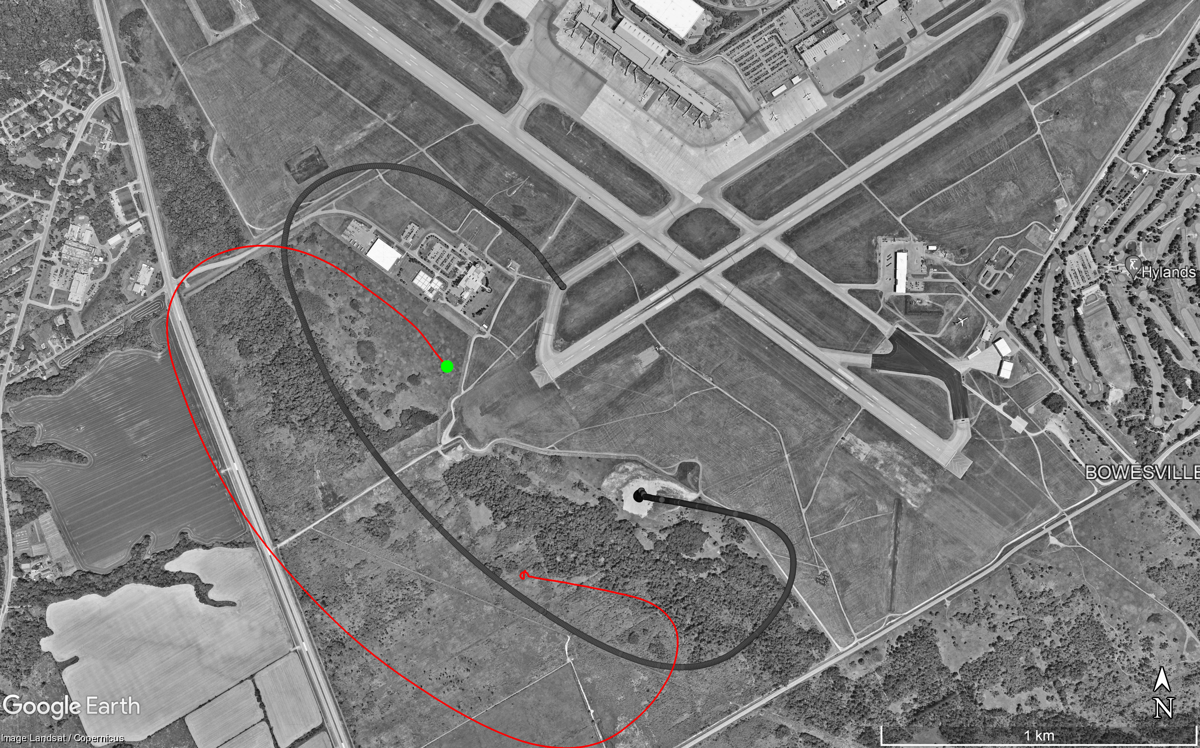
\includegraphics[width=\linewidth]{figures/track_on_map.png}
\caption{Georeferencing error in the shipped map metadata. Red: the flight track
projected using the published parameters. Dark curve: the true path, drawn onto
the map by the dataset authors. The two differ by 456\,m.}
\label{fig:trackmap}
\end{figure}

\subsection{Reference Imagery}

The shipped maps are unsuitable as a tile source for two further reasons: the
painted flight path is 18.6\,m wide on the ground and falls inside nearly every
tile a query could match to, and their resolution (0.79\,m/px) is coarser than
the queries. We therefore download Esri World Imagery \cite{esri2026} at zoom
level 19 (0.21\,m/px) covering the flight area.

The mapping from the local ENU frame to map pixels is obtained by least squares
against the PPK latitudes and longitudes, giving a residual of 0.30\,px
(0.06\,m). As an independent check, the PPK solution leads the bag timestamps by
exactly 18.00\,s, the GPS-to-UTC leap second count for 2022.

\begin{figure}[H]
\centering
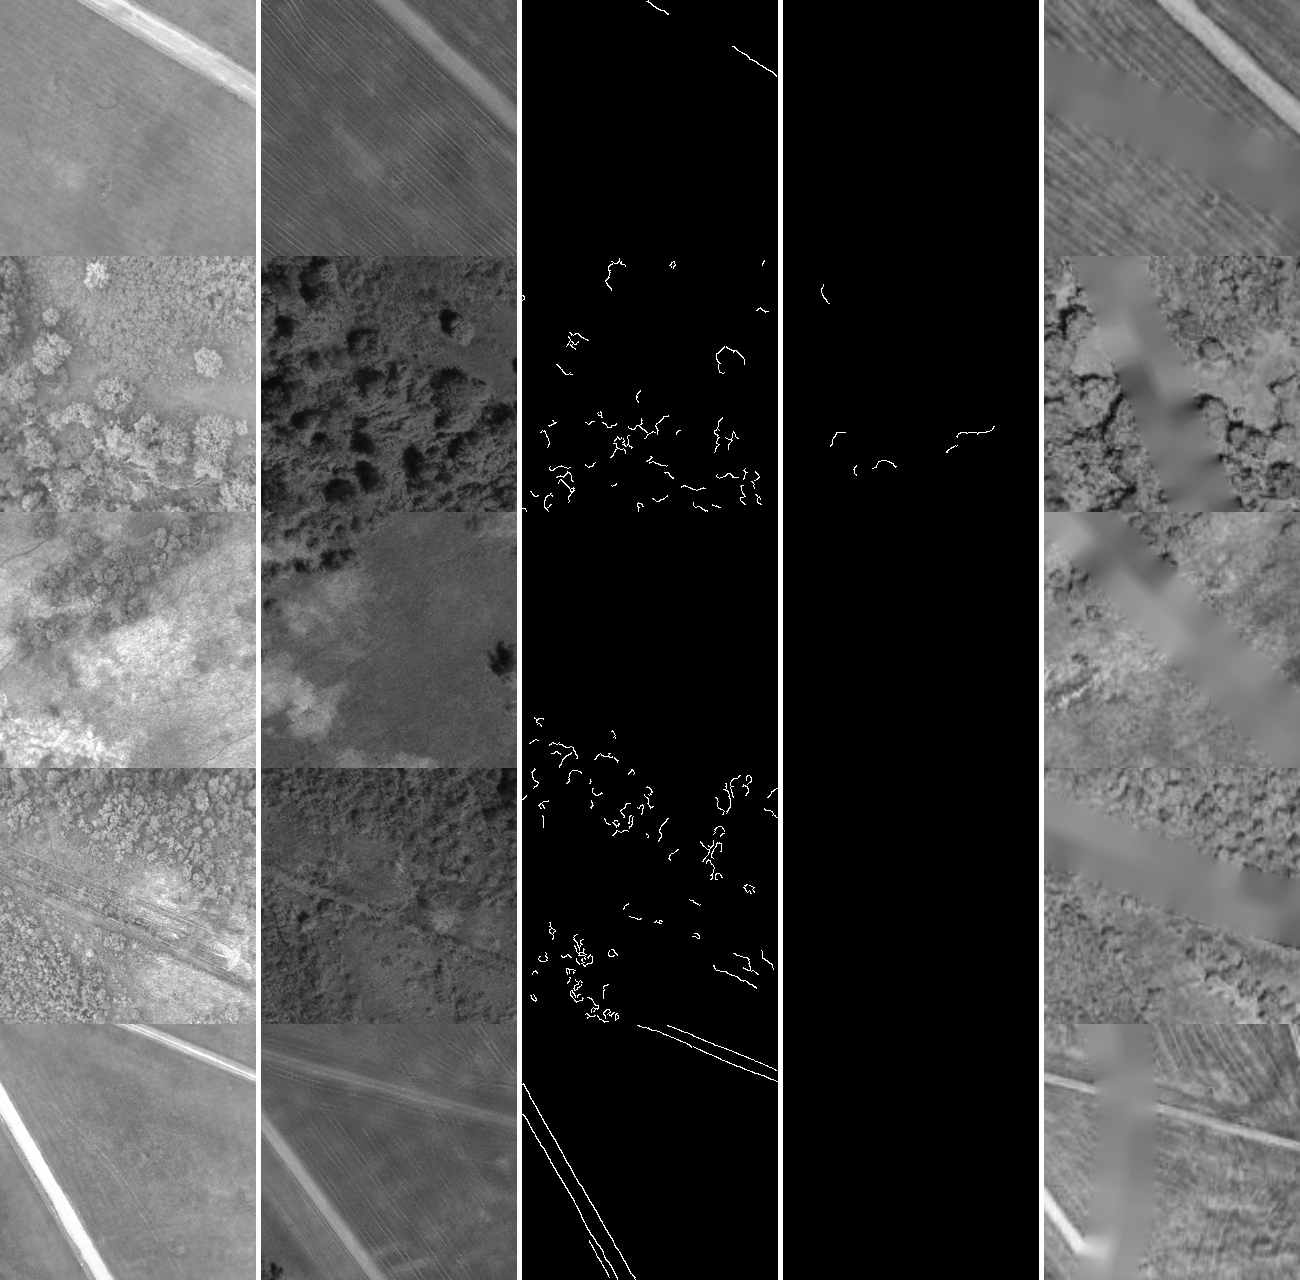
\includegraphics[width=\linewidth]{figures/esri_vs_munfrl.png}
\caption{Query, Esri tile, their Canny edge maps, and the corresponding
shipped-map tile. The fetched imagery yields 12.97\% edge density against the
camera's 16.75\%, compared with 5.38\% for the shipped map.}
\label{fig:esri}
\end{figure}

\subsection{Query Generation}

Map tiles cover a fixed ground extent, whereas a camera frame covers an area
proportional to altitude, so the two correspond only after resampling. Each
output pixel is treated as a point on the ground plane in ENU, rotated into the
camera frame through the full VIO attitude and the Kalibr
\cite{furgale2013kalibr} extrinsic, then projected through the equidistant
distortion model:
\begin{align}
\bm{P}_{\text{enu}} &= (\text{east},\ \text{north},\ z_{\text{ground}} - z_{\text{cam}}) \\
\bm{P}_{\text{imu}} &= \bm{R}_{G\rightarrow I}\, \bm{P}_{\text{enu}} \\
\bm{P}_{\text{cam}} &= \bm{R}_{C\rightarrow I}^{\top} (\bm{P}_{\text{imu}} - \bm{p}_{C\ \text{in}\ I}) \\
\bm{u} &= \pi_{\text{equi}}\!\left(\bm{P}_{\text{cam},xy} / \bm{P}_{\text{cam},z}\right)
\end{align}

Attitude must come from the VIO, since the PPK solution provides position only.
This is also the correct architecture: the VIO supplies attitude, and
geo-localization supplies position. Because OpenVINS initialises with an
arbitrary heading, the constant yaw offset between its frame and the map is
recovered by fitting the two tracks; this is an evaluation convenience and is
discussed as a limitation in Section~\ref{sec:limits}.

\section{Method}

\subsection{Visual-Inertial Odometry}

OpenVINS runs monocular with the nadir camera only. Online camera and IMU
intrinsic calibration is disabled, since the dataset provides Kalibr-grade
values. Anchored on the first 20\,s of flight, the estimate begins 14.7\,m from
truth and drifts to 700\,m by the end (Fig.~\ref{fig:anchor}), approximately
19\% of distance flown. A best-fit similarity transform reduces this to 215\,m,
indicating that the majority of the error is a systematic scale deficit of
approximately 40\% rather than accumulated random walk. The cause was not
identified; IMU restamping did not remove it.

\begin{figure}[H]
\centering
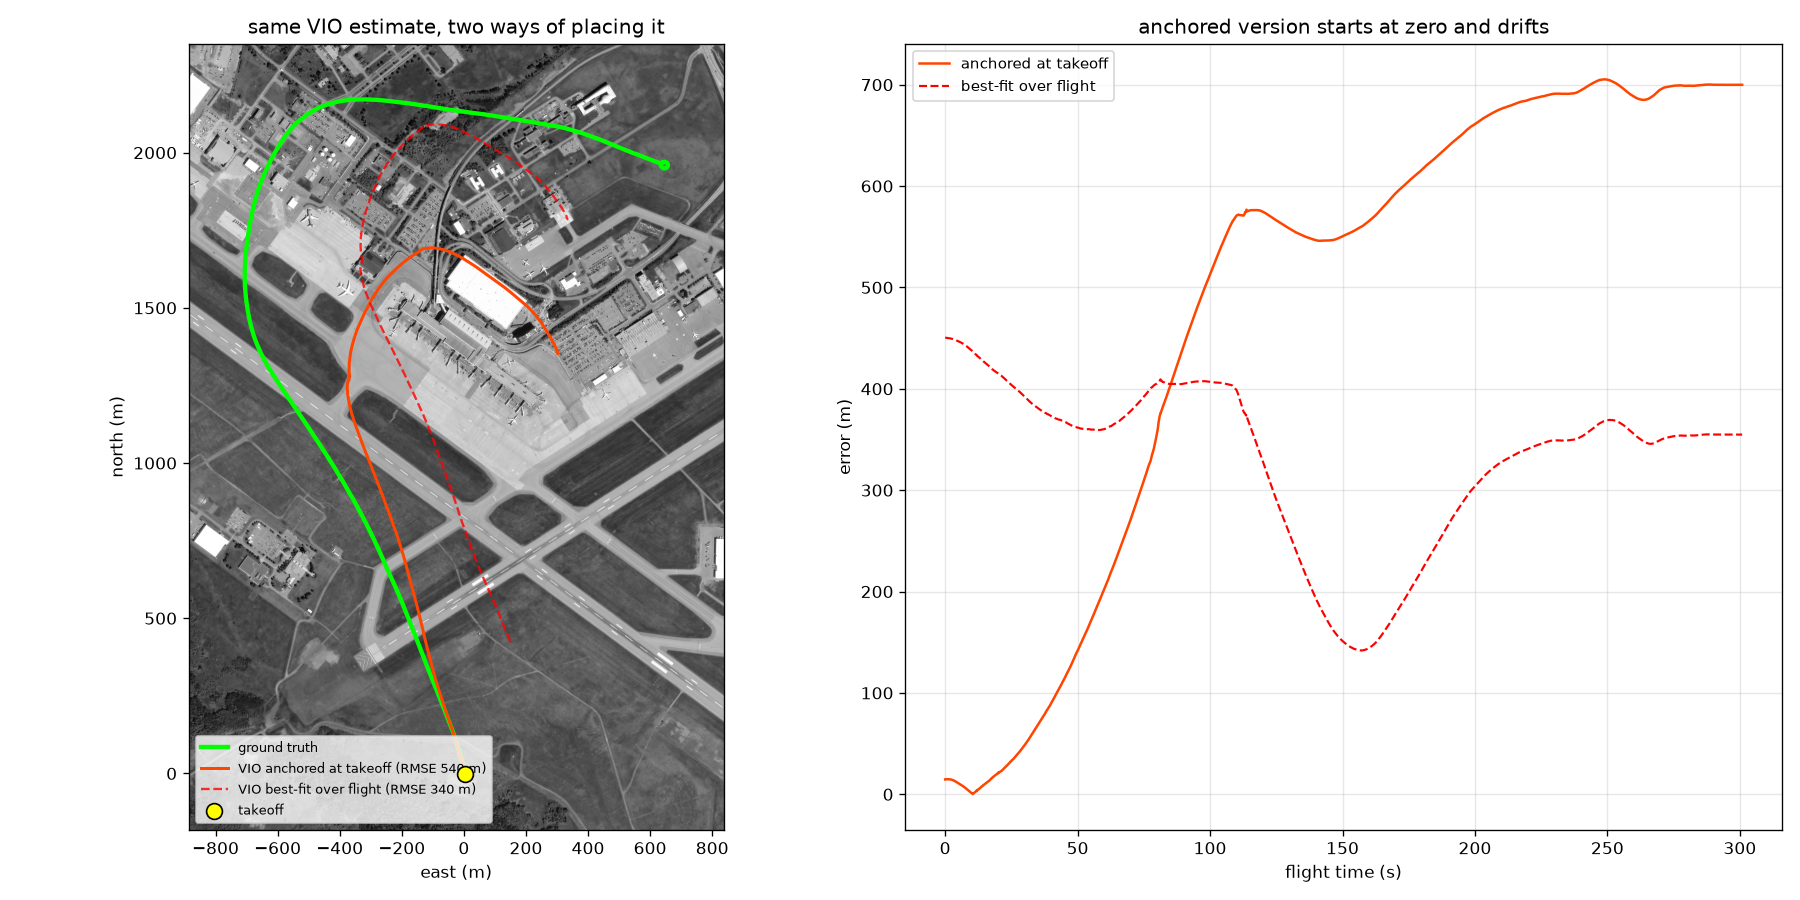
\includegraphics[width=\linewidth]{figures/vio_anchoring_dataset4.png}
\caption{OpenVINS anchored at takeoff (orange) starts on the truth and drifts to
700\,m. A best-fit placement over the whole flight (dashed) distributes the same
error differently.}
\label{fig:anchor}
\end{figure}

\subsection{Retrieval and Search Restriction}

Reference tiles are cut at a 100\,m ground footprint with 25\,m spacing and
encoded once offline into 1024-dimensional descriptors. Queries are matched by
cosine similarity.

Restricting the tile database to a corridor around positions where queries exist
--- rather than around the entire ground-truth track --- reduces the database
from 5340 to 1612 tiles and doubles recall
(Table~\ref{tab:retrieval}). We measured that 83\% of erroneous predictions
matched tiles more than 100\,m from any query position, i.e.\ tiles that could
never have been correct. In deployment this restriction corresponds to searching
within the uncertainty region defined by the motion prior, which is standard
practice for place recognition with odometry.

Reducing the tile footprint to 60\,m to admit lower-altitude frames was tested
and \emph{degrades} performance: recall falls to 13.6\%. Descriptor analysis
shows why --- at 60\,m, 2.21\% of tile pairs exceed 0.99 cosine similarity
against 0.31\% at 100\,m, so distinct locations become indistinguishable. This
places a lower bound on usable tile size for this terrain.

\begin{table}[H]
\centering
\caption{Retrieval on \texttt{bell412\_dataset4}. R@100\,m is the fraction of
queries whose top-1 tile lies within 100\,m of the true position.}
\label{tab:retrieval}
\begin{tabular}{@{}lcccc@{}}
\toprule
Configuration & Tiles & R@100\,m & Median err. & ms/query \\
\midrule
100\,m tile, 400\,m corridor & 5340 & 17.7\% & 406\,m & 229 \\
100\,m tile, 200\,m corridor & 1612 & \textbf{35.8\%} & \textbf{230\,m} & 233 \\
60\,m tile, 200\,m corridor  & 3270 & 13.6\% & 476\,m & 235 \\
\bottomrule
\end{tabular}
\end{table}

Runtime is unaffected by database size (229--235\,ms across a 3.3$\times$ range),
confirming that cost is dominated by encoding the query rather than searching
the map.

\subsection{The Confidence Score is Not Informative}
\label{sec:score}

Measured over both available flights, the cosine similarity of the retrieved
match is \emph{slightly negatively} correlated with correctness: on
\texttt{dataset4} the mean score is 0.9429 for correct predictions and 0.9493
for incorrect ones; on \texttt{dataset3}, 0.9447 against 0.9598. The 60\,m
experiment explains the mechanism --- descriptor collapse produces near-perfect
similarity precisely when tiles are least distinguishable.

Consequently no threshold on the retrieval score can separate inliers from
outliers, and gating must rely on geometry instead.

\subsection{Consensus-Based Outlier Rejection}

Incorrect predictions are distributed approximately uniformly over the
tile database, so the probability that two independent errors land near the same
place --- after accounting for the VIO displacement between their timestamps ---
is well below 1\%. Mutual agreement is therefore strong evidence of correctness,
and it is available without reference to any filter state.

Within a sliding window of predictions, RANSAC \cite{fischler1981ransac}
hypothesises a similarity transform from two predictions and their corresponding
VIO positions, scoring it by how many other predictions in the window it
explains. Predictions belonging to the largest consistent set are retained.

\begin{table}[H]
\centering
\caption{Consensus rejection on \texttt{bell412\_dataset4}.}
\label{tab:consensus}
\begin{tabular}{@{}lcc@{}}
\toprule
 & Before & After \\
\midrule
Predictions & 299 & 101 \\
Precision & 17.7\% & \textbf{99.0\%} \\
Median error of retained & --- & 17\,m \\
Correct predictions retained & 107 & 100 (93\%) \\
\bottomrule
\end{tabular}
\end{table}

\begin{figure}[H]
\centering
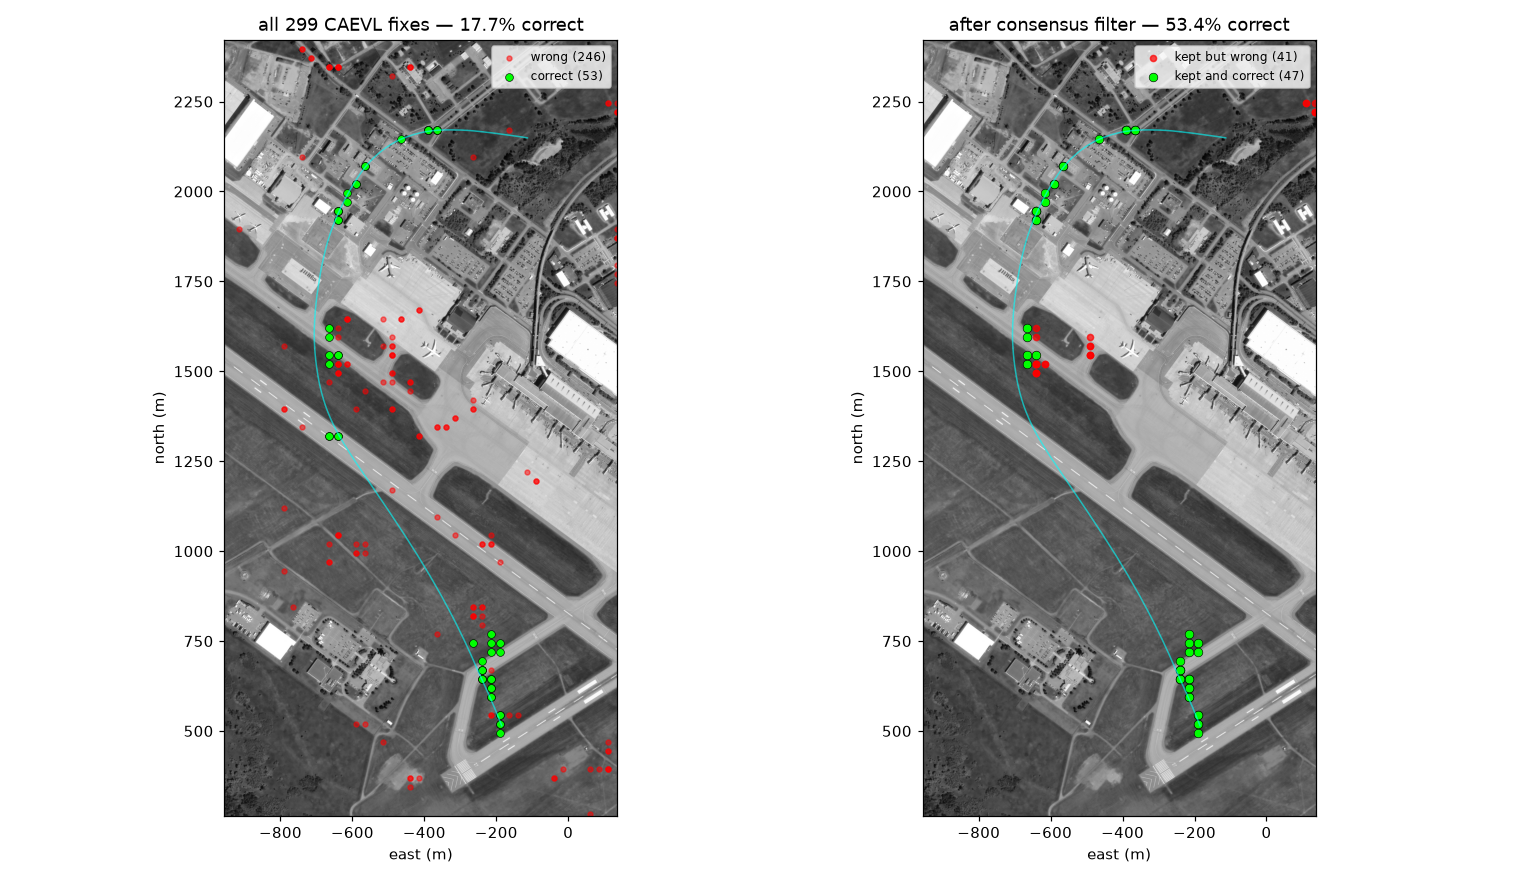
\includegraphics[width=\linewidth]{figures/consensus_filter.png}
\caption{Consensus rejection. Left: all predictions, green correct, red
incorrect. Right: after filtering. Precision rises from 17.7\% to 99.0\% while
93\% of correct predictions survive.}
\label{fig:consensus}
\end{figure}

\subsection{Causal Fusion}

The fused estimate is the VIO trajectory mapped into the map frame by a
similarity transform $(s, \theta, \bm{t})$ estimated online from accepted
predictions:
\begin{equation}
\hat{\bm{p}}_k = s\, \bm{R}(\theta)\, \bm{p}^{\text{vio}}_k + \bm{t}
\end{equation}

Estimating $s$ is essential rather than optional: OpenVINS initialises with an
arbitrary heading, and its 40\% scale deficit would otherwise reappear between
every pair of predictions.

The estimator is strictly causal. A prediction enters a buffer when its
timestamp elapses; a \emph{trailing} window of that buffer is screened for
consensus; survivors accumulate; and the transform is refitted by
Umeyama's method \cite{umeyama1991} to all predictions accepted so far. Scale is
observable only over long baselines, so the fit uses the full accepted history
rather than a short window --- still causal, with growing memory. Until enough
accepted predictions span 300\,m no transform exists and the system is simply
not localised; this warm-up is reported rather than concealed.

An extended Kalman filter over $(x, y, s, \theta)$ with chi-square gating was
also implemented and performs substantially worse (392\,m for the transform
estimator against 422\,m for the EKF). Two reasons: the filter must judge each
prediction on arrival using only its current belief, whereas consensus examines a
window jointly; and a per-prediction position update allows position to absorb
the innovation, leaving scale to converge too slowly. The EKF is retained in the
implementation for comparison.

\section{Results}

\begin{table}[H]
\centering
\caption{Fusion on \texttt{bell412\_dataset4}, both trajectories anchored at
takeoff. Causal uses only information available at each instant.}
\label{tab:fusion}
\begin{tabular}{@{}lccc@{}}
\toprule
 & OpenVINS & Fused & Reduction \\
\midrule
\textbf{Causal (real-time)} & & & \\
\quad RMSE & 617\,m & \textbf{392\,m} & 36\% \\
\quad Final error & 700\,m & 515\,m & 26\% \\
\midrule
\textbf{Offline (upper bound)} & & & \\
\quad RMSE, whole flight & 452\,m & 314\,m & 31\% \\
\quad RMSE, cruise only & 166\,m & \textbf{48\,m} & 71\% \\
\bottomrule
\end{tabular}
\end{table}

\begin{figure}[H]
\centering
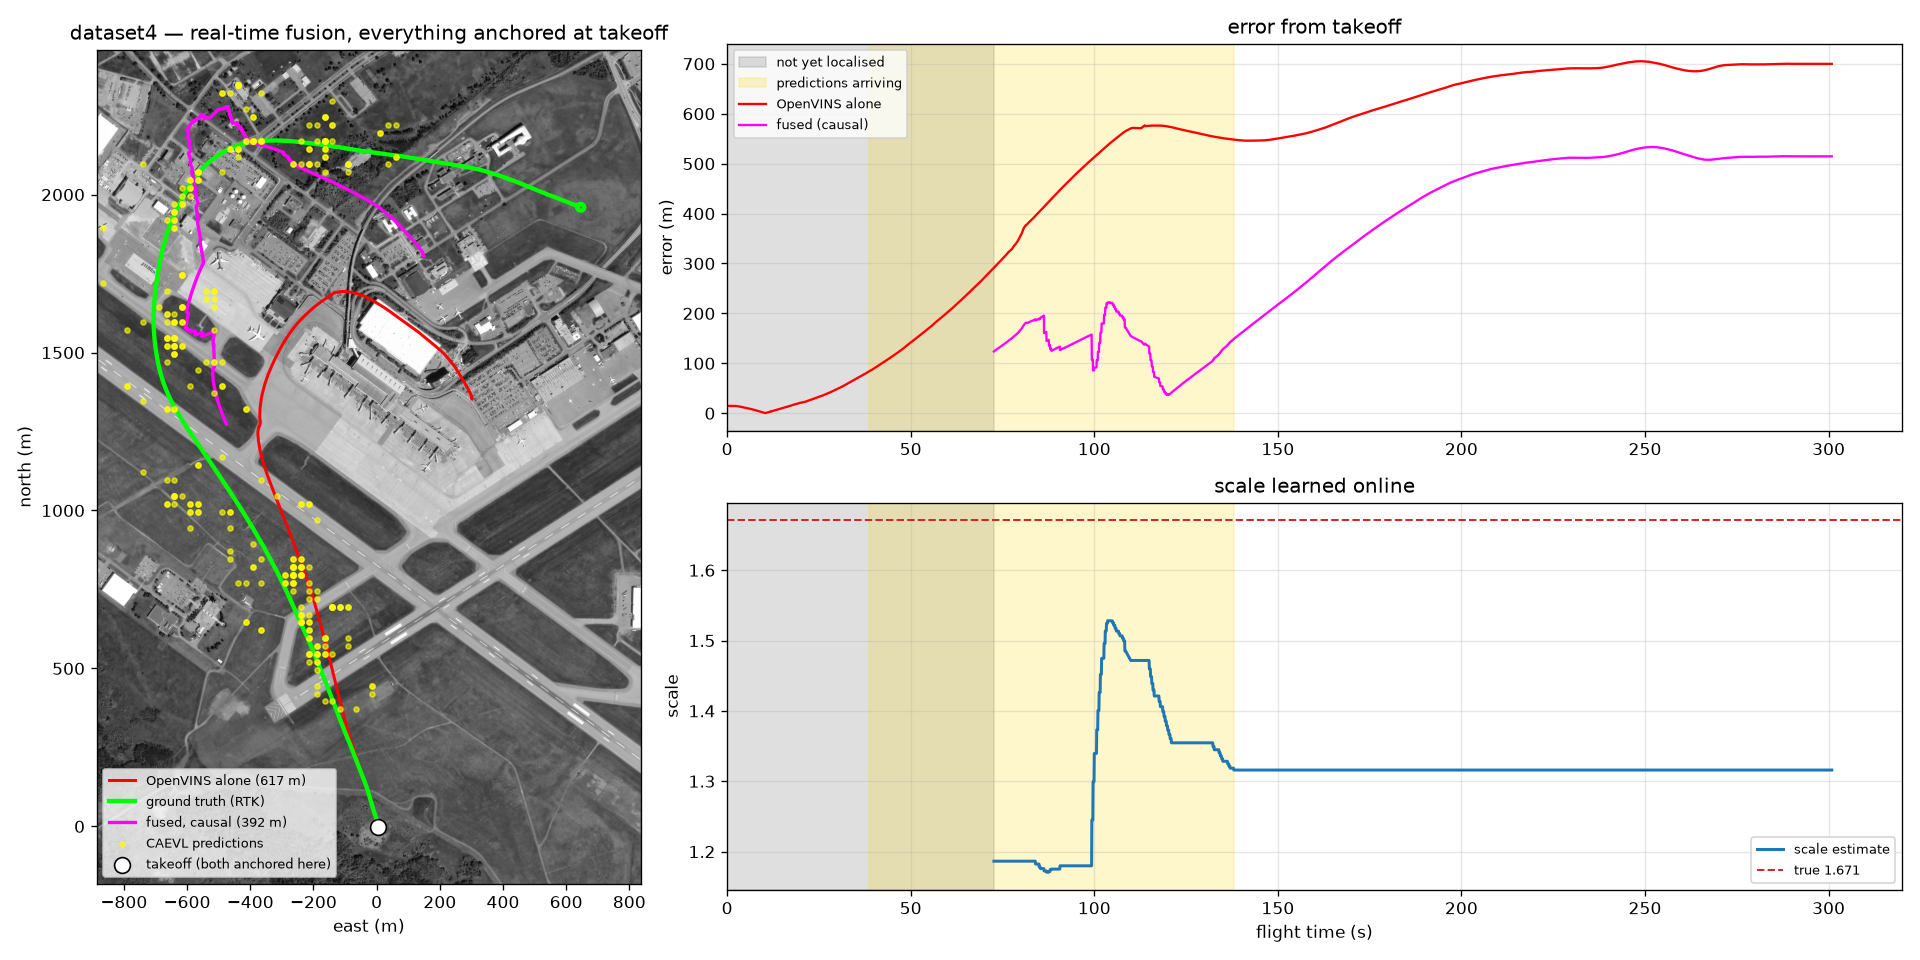
\includegraphics[width=\linewidth]{figures/FINAL_causal_dataset4.png}
\caption{Causal fusion. Red: OpenVINS alone. Green: RTK ground truth. Magenta:
fused. Yellow: CAEVL predictions. Grey band: before localisation is available.
Gold band: while predictions arrive. Bottom right: the online scale estimate,
which does not fully converge before predictions cease.}
\label{fig:causal}
\end{figure}

The gap between the causal and offline results is itself informative. The
offline estimator may use predictions from $t=152$\,s to correct the estimate at
$t=60$\,s; a deployed system cannot. Its scale estimate reaches only 1.32 of the
required 1.671 before predictions stop, so the correction is partial. With
absolute fixes available across a larger fraction of the flight, scale would
converge earlier and the causal result would approach the offline one.

\subsection{Terrain Dependence}

The same pipeline applied to \texttt{bell412\_dataset3} --- the same aircraft,
the same airport, the same network weights --- yields R@100\,m of 8.9\% against
17.7\% under identical settings. The difference is what the camera observes:
\texttt{dataset3} loops over continuous forest canopy, whereas
\texttt{dataset4} crosses the terminal apron, hangars and taxiways.
Fig.~\ref{fig:where} shows correct predictions clustering on man-made structure
and failing over uniform ground. Over forest, Canny edge maps are texture noise
and every tile resembles every other.

\begin{figure}[H]
\centering
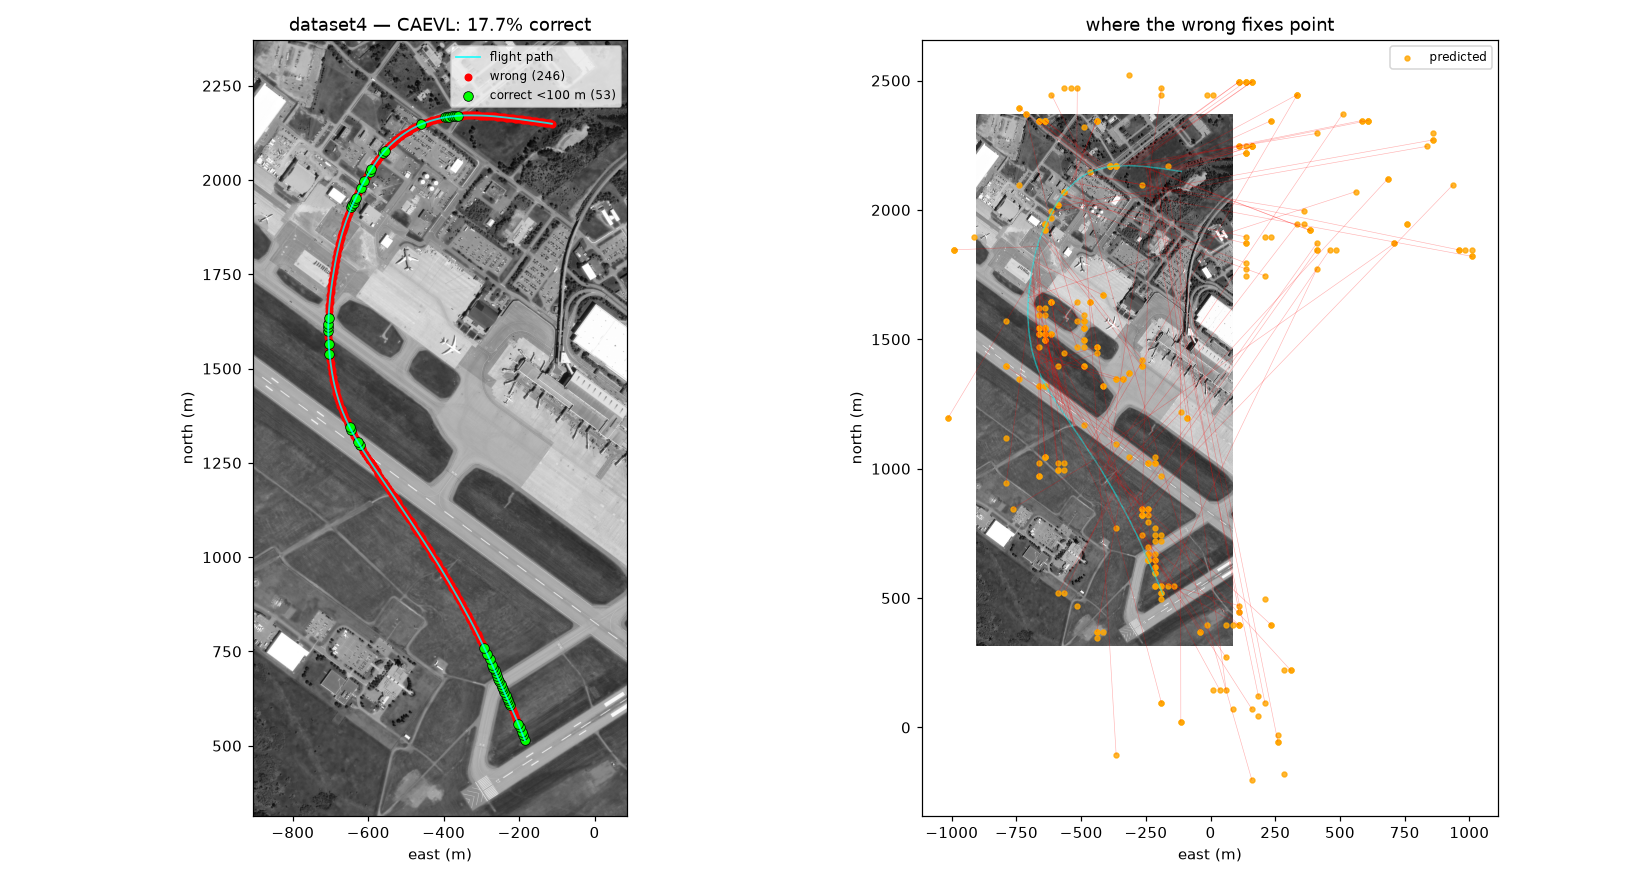
\includegraphics[width=\linewidth]{figures/caevl_dataset4_map.png}
\caption{Where retrieval succeeds. Green: correct within 100\,m. Red:
incorrect. Successes concentrate on runway markings and the terminal apron.}
\label{fig:where}
\end{figure}

\section{Limitations}
\label{sec:limits}

\textbf{Altitude coverage is the dominant constraint.} A 100\,m tile requires
approximately 66\,m of altitude to be fully imaged, since the camera observes
about $1.5\times$ its height in ground extent. Only 34\% of this flight is flown
above that threshold: the profile is takeoff, a 70\,s cruise near 105\,m,
descent, and then 80\,s of level flight at approximately 11\,m where the camera
images 17\,m of ground. No map-matching method can localise from that. The
restriction is physical, not algorithmic --- and reducing tile size to
compensate fails, as shown in Section~\ref{tab:retrieval}.

\textbf{Two quantities are taken from ground truth.} Query generation uses the
ground-truth altitude to normalise ground extent, and the VIO-to-map yaw offset
is obtained by fitting the two tracks. Both are evaluation conveniences. In
deployment, altitude would come from a barometric or radar altimeter --- standard
equipment that MUN-FRL does not record --- and the initial heading from a
magnetometer or the first accepted prediction. We verified that the VIO's own
altitude is not an adequate substitute: its median error against truth is
29.8\,m, which at 100\,m altitude corresponds to a 30\% error in the ground
extent of every query.

\textbf{Single flight fused.} Retrieval was evaluated on two sequences, but the
fusion result is reported for one.

\textbf{The VIO scale deficit is unexplained.} A systematic 40\% shortfall is
larger than expected for a well-calibrated visual-inertial system and was not
resolved by IMU restamping.

\section{Conclusion}

We have demonstrated a CPU-only pipeline that bounds VIO drift using
self-supervised aerial geo-localization requiring no paired training data,
evaluated on real flight data with centimetre-accurate ground truth. In
real time, position RMSE falls from 617\,m to 392\,m; where absolute fixes are
available, offline error falls from 166\,m to 48\,m.

The principal finding is methodological: with an inlier rate below 20\% and a
confidence score that is negatively correlated with correctness, the decision of
\emph{which} absolute measurements to accept matters more than the estimator that
consumes them. Consensus among temporally adjacent predictions, evaluated
through the motion prior, raises precision from 17.7\% to 99.0\% while retaining
93\% of correct predictions, and does so without consulting either the retrieval
score or the filter's own belief --- avoiding the divergence failure mode in
which a drifted filter rejects precisely the measurements that would correct it.

The limiting factor is availability rather than accuracy. Future work should
address altitude coverage directly: query-side scale normalisation in the manner
of Shao et al.\ \cite{shao2026altitude}, who construct a single-scale reference
database at the lowest operating altitude and rescale queries down to it, is the
most promising direction, together with retraining CAEVL at a tile footprint
matched to the deployment altitude rather than the 14.4$\times$ larger footprint
of its current training data.

\printbibliography

\end{document}
